\documentclass[10pt]{beamer}

\usetheme[numbering=none]{metropolis}
\usepackage{appendixnumberbeamer}

\usepackage[utf8]{inputenc}

\usepackage{booktabs}
\usepackage[scale=2]{ccicons}

\usepackage{verbatim}

\usepackage{pgfplots}
\usepgfplotslibrary{dateplot}

\usepackage{xspace}
\newcommand{\themename}{\textbf{\textsc{metropolis}}\xspace}


\title{Valaris}
\subtitle{Echtzeit Computergrafik in der Spieleentwicklung}
\date{28. August 2018}
\author{Artur Wesner}
\titlegraphic{\hfill\includegraphics[height=2.5cm]{./Bilder/ValarisLogo.png}}

\begin{document}

\maketitle

\begin{frame}{Qualitätsziele}
  \begin{itemize}
    \item Korrektheit
    \item Robustheit
    \item Benutzerfreundlichkeit
    \item Effizienz
    \item Optik 
  \end{itemize}
\end{frame}

\begin{frame}{Testtools}
    \begin{itemize}
        \item JUnit für automatische Tests
        \item Coverage nur teilweise möglich gewesen
        \item Manuelle Tests 
        \item Profiler zum Anzeigen der fps
        \item Taskmanager für Speicherauslastung
        \item Roadmodalrenderer für Modellierung der erzeugten Strecke
      \end{itemize}
\end{frame}

\begin{frame}[standout]{}
    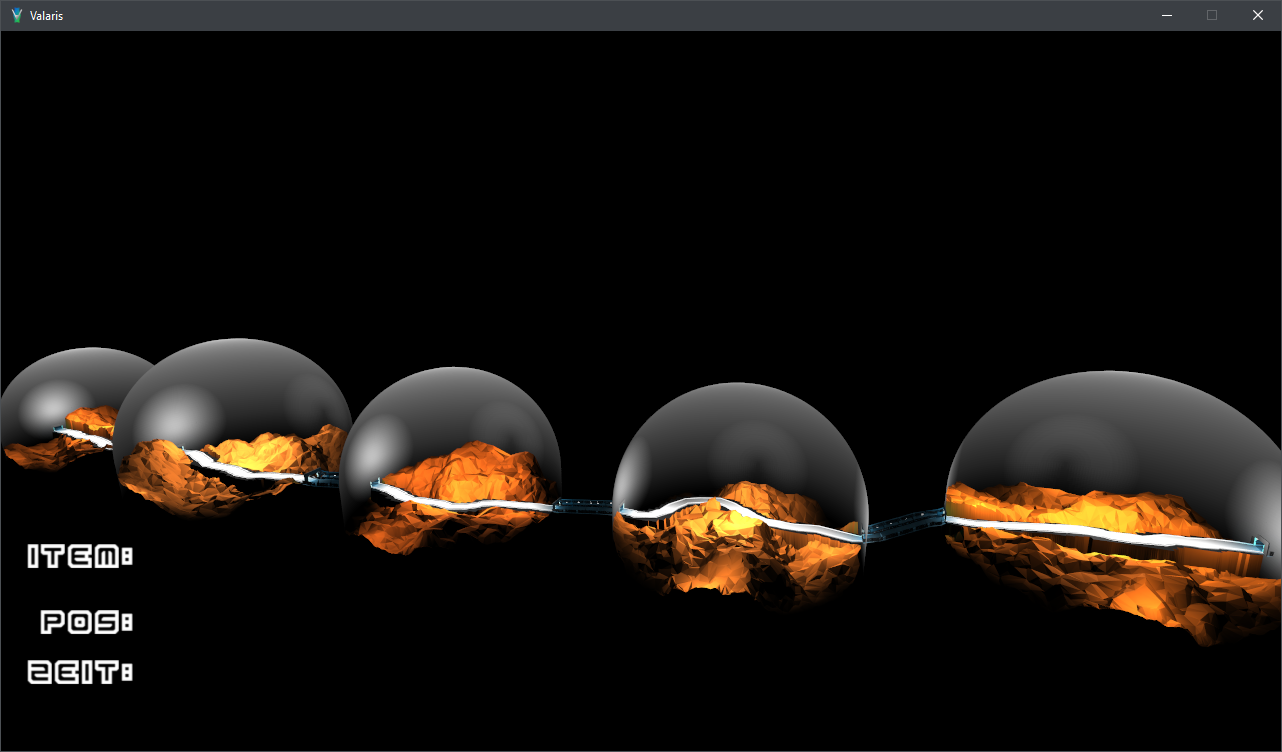
\includegraphics[width=\textwidth]{./Bilder/canyons.png}\\
\end{frame}

\begin{frame}[standout]{}
    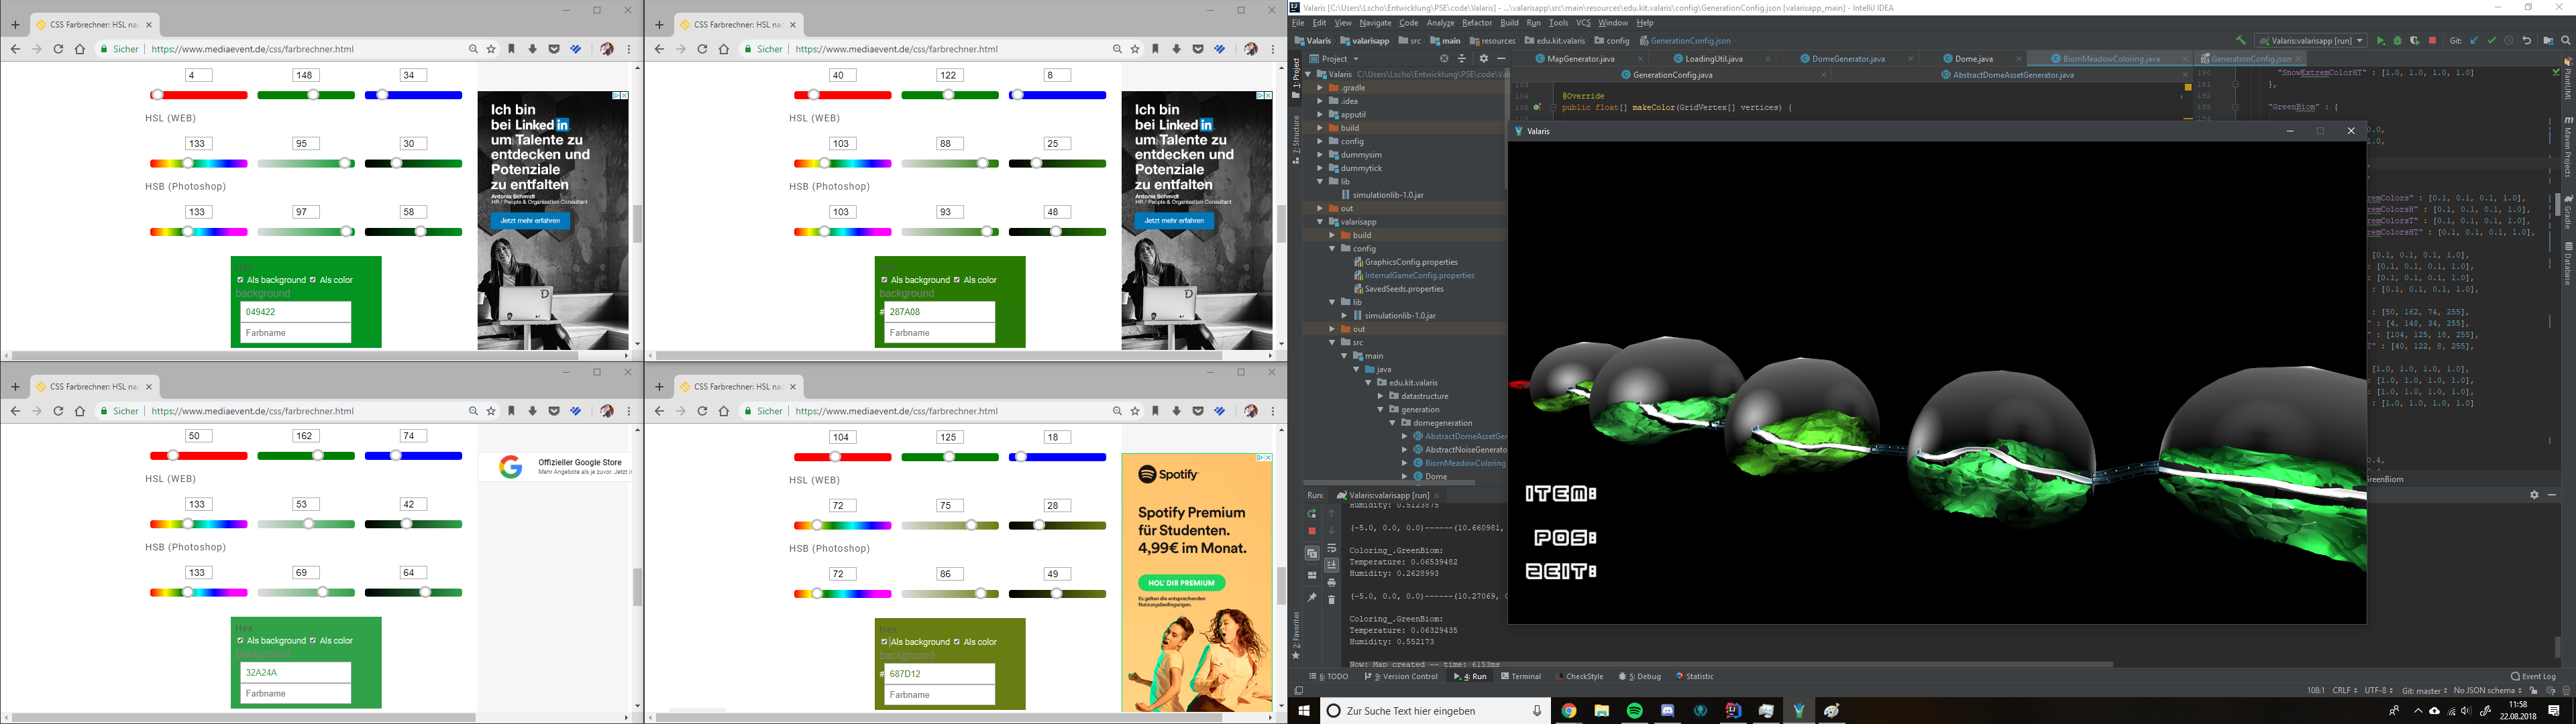
\includegraphics[width=\textwidth]{./Bilder/GreenBiomsCreating.png}\\
\end{frame}

\begin{frame}[standout]{}
    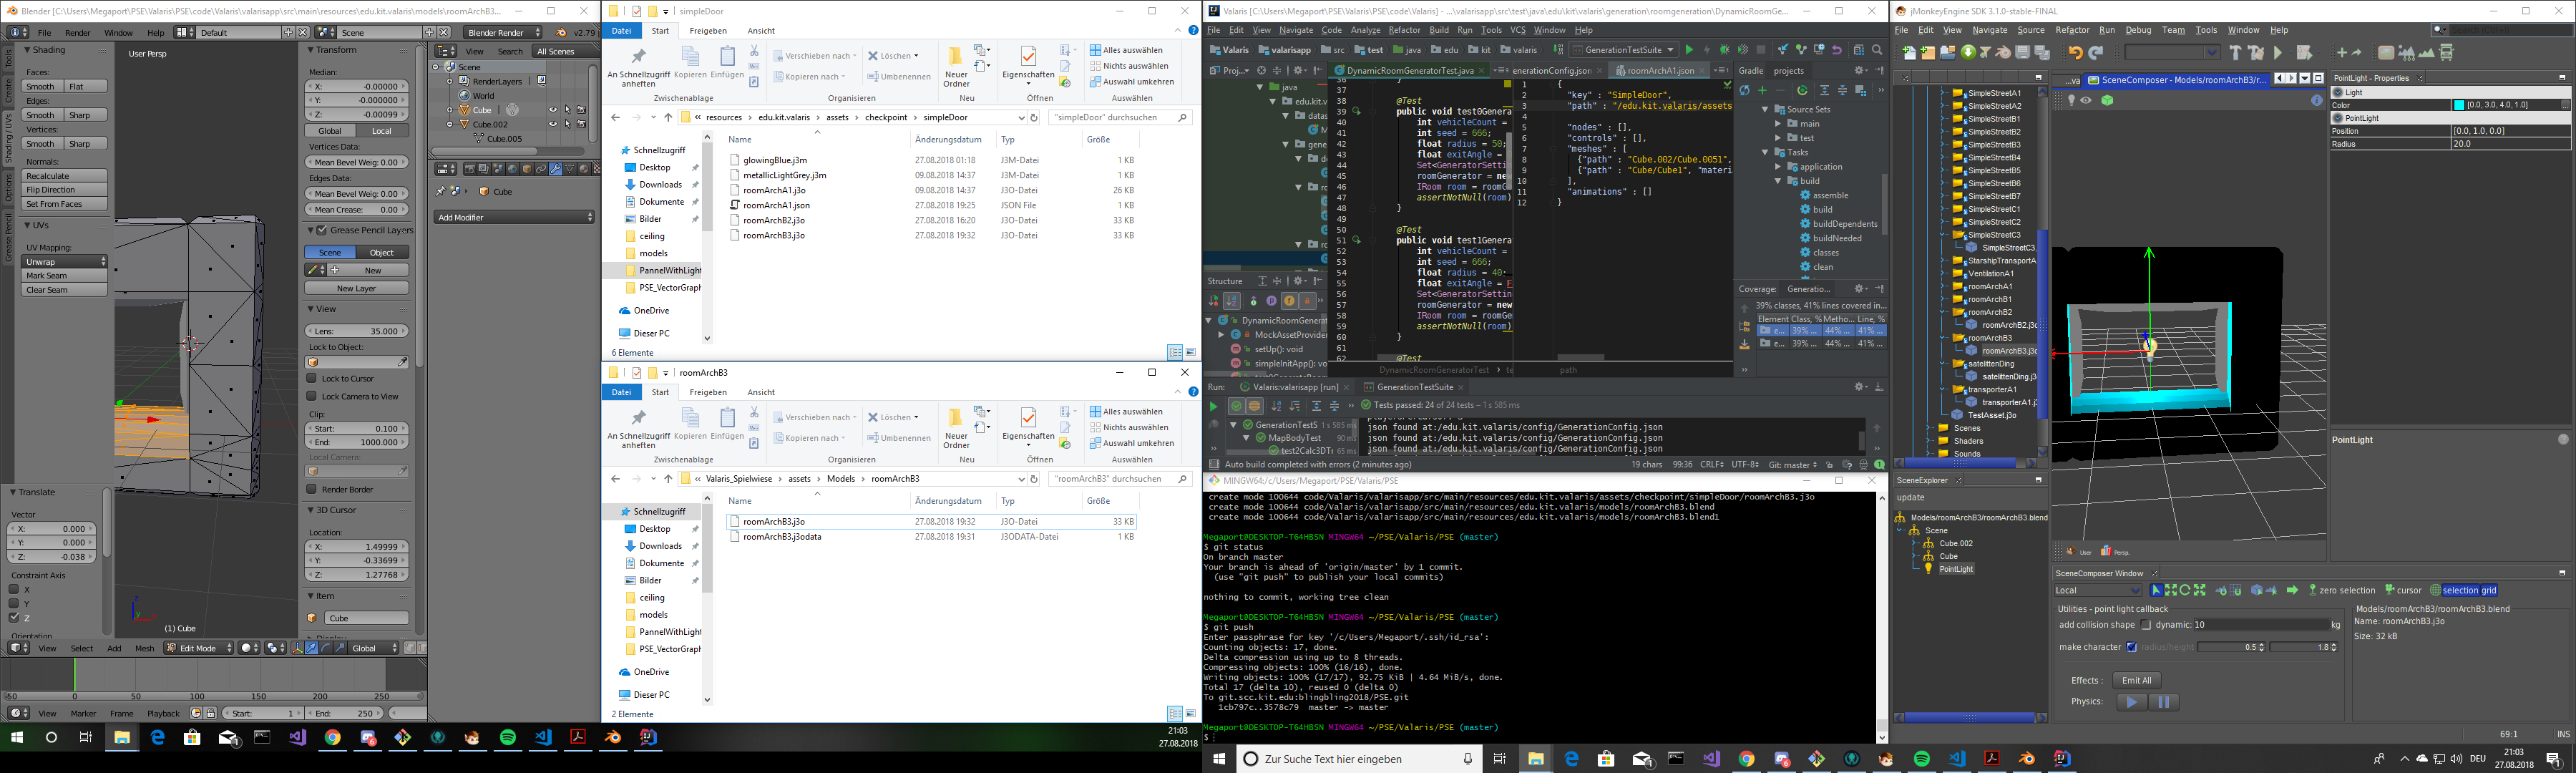
\includegraphics[width=\textwidth]{./Bilder/assetErstellungsChaos.png}\\
\end{frame}

\begin{frame}{Wichtigsten Änderungen/Features}
    \begin{itemize}
        \item Erweiterung der Assets, Bepflanzung uvm.
        \item Parallelisierung der Generierung vom SceneGraph
        \item Vernünftige Platzierung von Objekten
        \item Console, mit der unsere eigene Simulation gestartet werden kann
        \item Verschönerung des Menüs
        \item Alle Menüs funktionieren und sind korrekt in das System integriert
    \end{itemize} 
\end{frame}

\begin{frame}{Probleme bei der Fehlerbehebung}
    \begin{itemize}
        \item Mapbody
        \item Inkontinuierlche Rotation behoben
        \item Partikeleffekte /-farben behoben/verbessert
        \item Culling Manager
        \item Korrektes Zusammenspiel von Menü+System
        \item Testergebnisse aus dem Pflichtenheft positiv
    \end{itemize}
\end{frame}

\begin{frame}{Statistiken}
    \begin{itemize}
        \item Klassen: 134
        \begin{itemize}
            \item Controls: 2
            \item Assets: 16
            \item Console: 1
            \item Profiling: 5
            \item Threading: 2
            \item DummySimulation: 2
            \item Datastructure: 2
            \item Generation: 38
            \item Menu: 24
            \item Rendering: 39
        \end{itemize}
        \item SourceCode: 24.392
        \item SourceCode(von uns erstellt): 23.118
        \item JavaCode: 13.726
        \item JavaCode(von uns erstellt): 13.200
        
    \end{itemize}
\end{frame}

%\appendix
\end{document}